\documentclass[a4]{scrartcl}

% \usepackage[ngerman]{babel}
\usepackage[utf8]{inputenc}
\usepackage{mathtools}
\usepackage{amsmath}
\usepackage{amssymb}
\usepackage{geometry}
\usepackage{scrlayer-scrpage}
\usepackage{float}
\usepackage{xcolor}
\pagestyle{scrheadings}
\clearscrheadfoot

\usepackage[backend=biber, maxbibnames=99]{biblatex}
\addbibresource{references.bib}

\setlength{\parindent}{0cm}


\geometry{
  paper=a4paper, % Change to letterpaper for US letter
  top=2cm, % Top margin
  bottom=1.5cm, % Bottom margin
  left=2cm, % Left margin
  right=3cm, % Right margin
}

\ohead{\\
Pina Kolling\\
piko0011}

\usepackage[framemethod=TikZ]{mdframed}

% Style %
\mdfdefinestyle{enviStyle}{
   innertopmargin = 10pt,
  linewidth      = 1pt,
  frametitlerule = true,
  roundcorner    = 2pt%
}


\newenvironment{CountingDefinition}[2][]{%
   \ifstrempty{#1}%
   {\mdfsetup{%
      frametitle={{\strut ~}}}
   }%
   {\mdfsetup{%
      frametitle={{\strut ~#1}}}%
   }%
   \mdfsetup{
      nobreak                   = true,
     linecolor                 = gray,
    frametitlebackgroundcolor = gray!50,
    style                     = enviStyle
   }
   \begin{mdframed}[]\relax%
   \label{#2}}{\end{mdframed}}

\begin{document}

\section*{Summary: Lecture 5}

Summary for the chapters \textit{X} and \textit{X}. \cite{book}







%-------------------------------------------------------------



\subsection*{Reduction}


\begin{minipage}{0.56\textwidth}
\textbf{Examples of NP-problems:}
\begin{itemize}
\item Travelling Salesman Problem
\item SATISFIABLE
\item REACHBILITY (in P)
\item CIRCUIT VALUE (in P)
\end{itemize}

\end{minipage}\begin{minipage}{0.4\textwidth}

\begin{figure}[H]
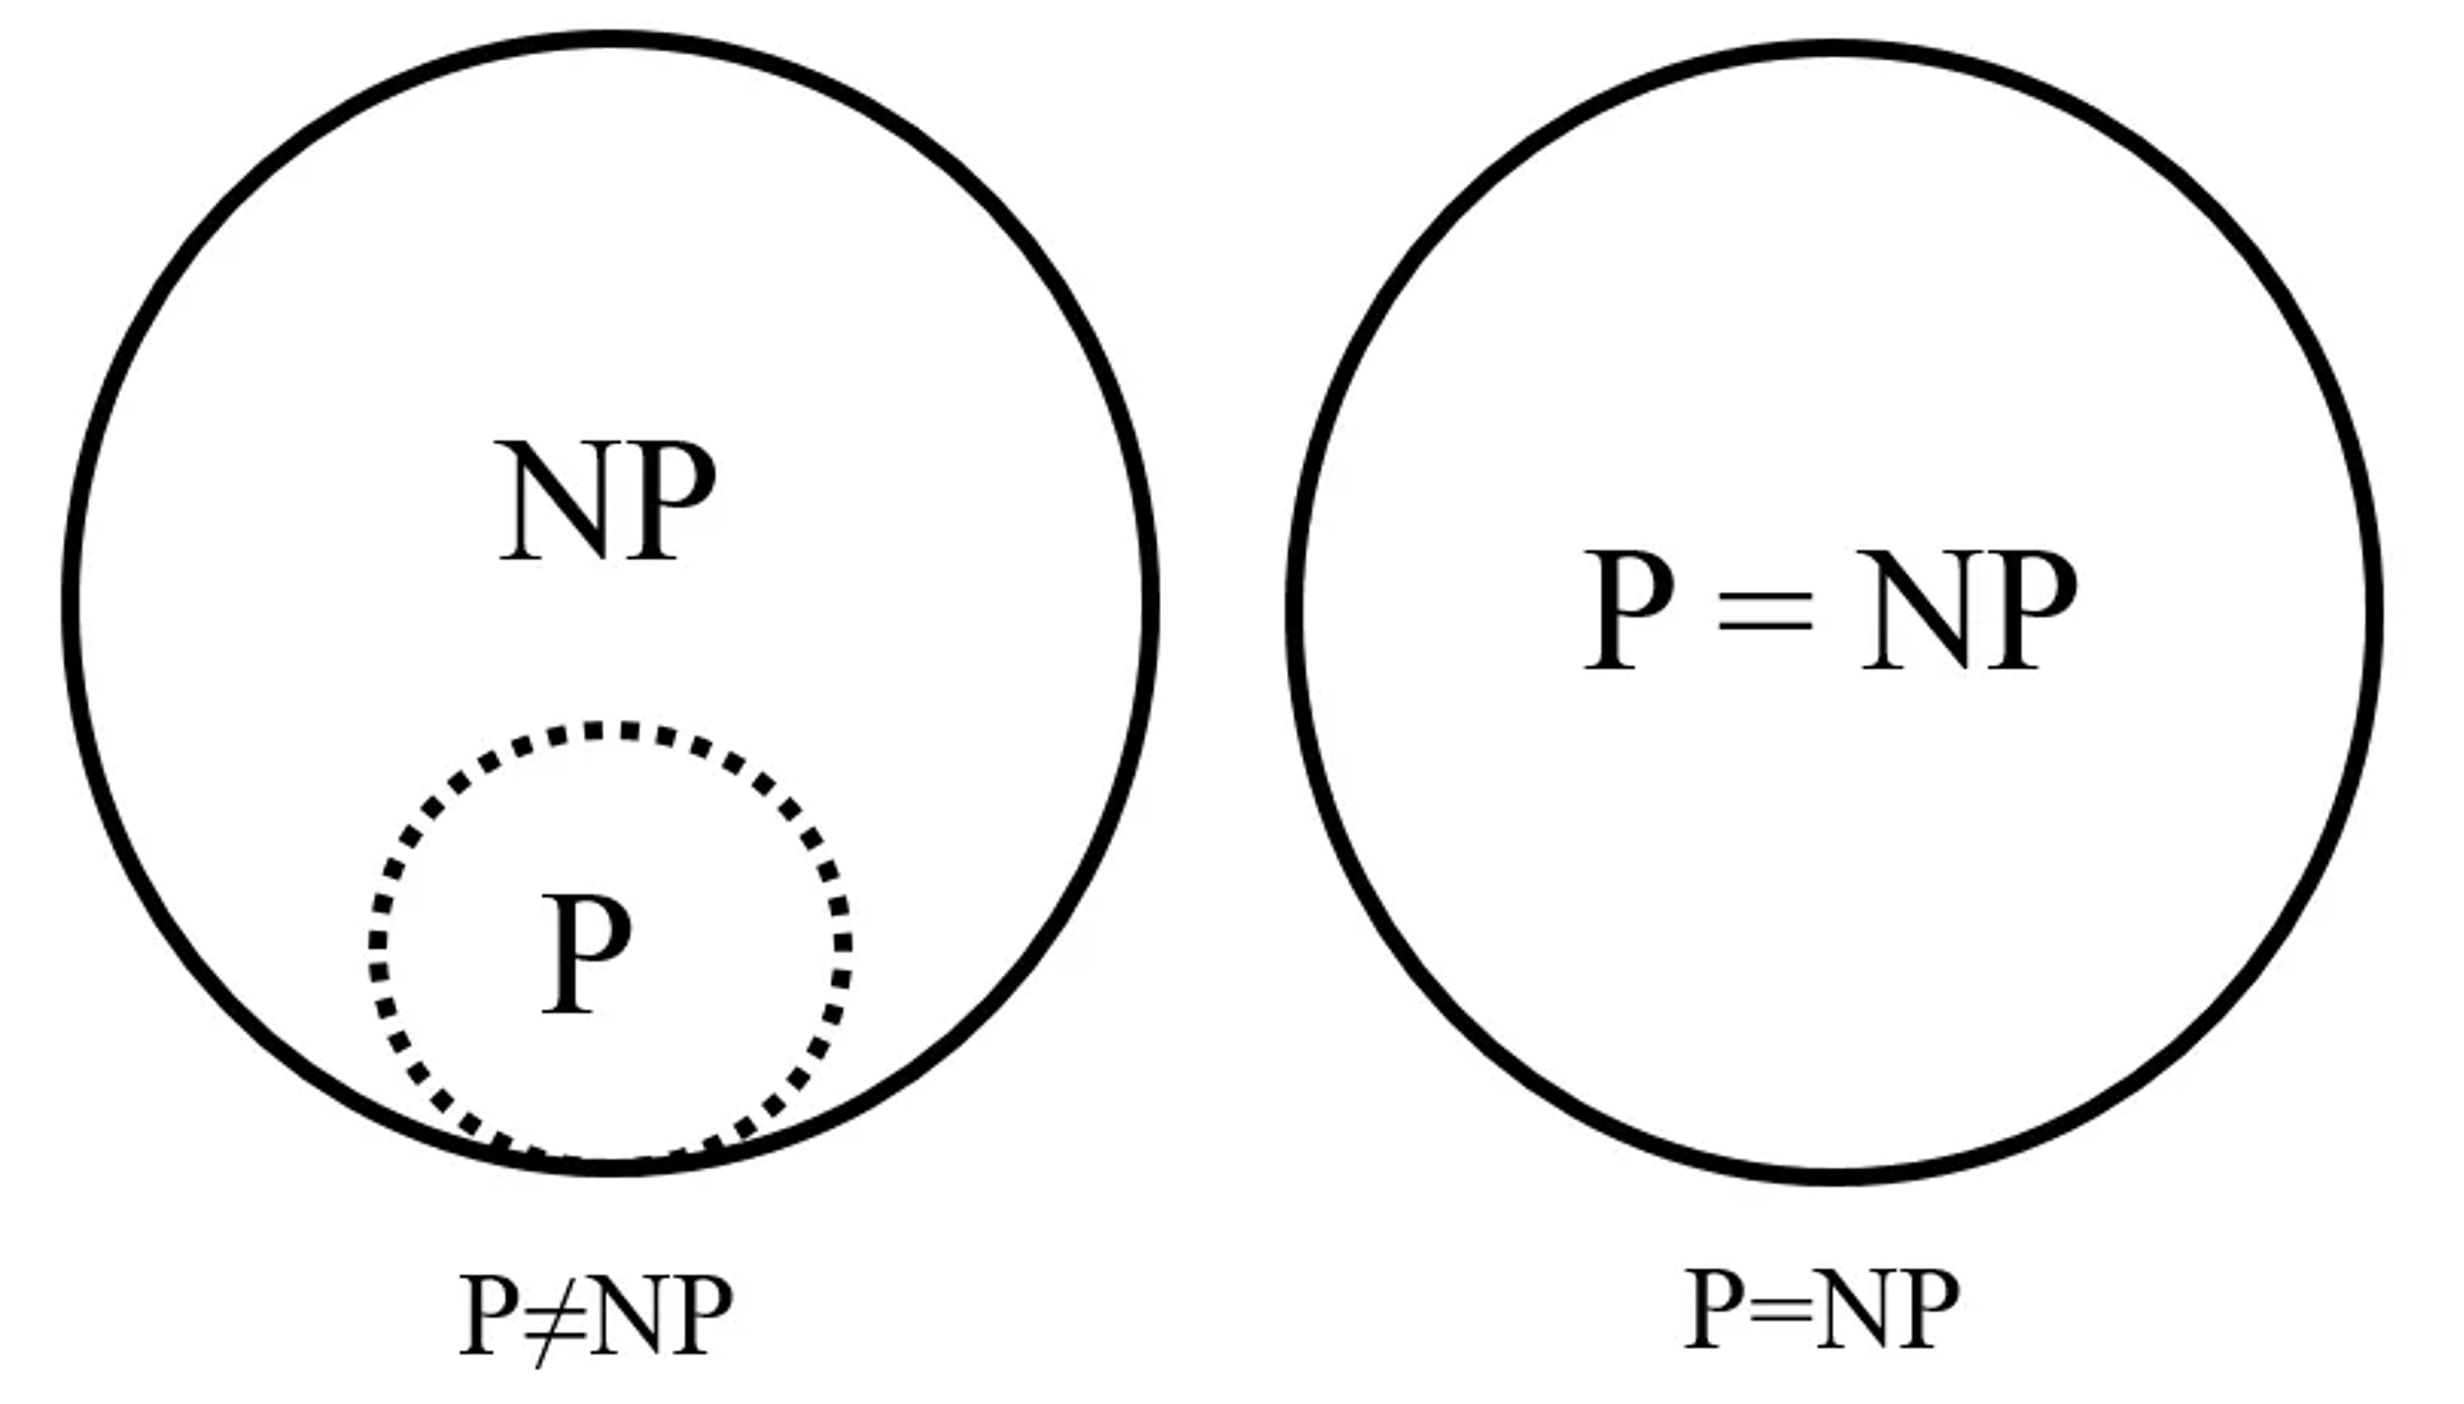
\includegraphics[scale=0.2]{PNP.jpg}
\caption{P and NP sets \cite{PNPsets}}
\end{figure}

\end{minipage}




\begin{itemize}
\item reduction: a problem is at least as hard as another
\item problem $A$ is at least as hard as problem $B$ if $B$ reduces to $A$
\item $B$ reduces to $A$ if there is a transformation $R$
\begin{itemize}
\item $R$ produces for every input $x$ of $B$ an equivalent input $R(x)$ of $A$ 
\item the answer of input $x$ on $B$ and input $R(x)$ on $A$ have to be the same
\end{itemize}
\item to solve $B$ on input $x$, $A$ can be solved instead with input $R(x)$
\end{itemize}

\begin{CountingDefinition}[Reduction]{def:validLabelPlacement}
Problem $A$ is at least as hard as problem $B$ if $B$ reduces to $A$.
\end{CountingDefinition}

\textbf{Transformation function:}
\begin{itemize}
\item tranformation function $R$ should not be too hard to compute \\
$\rightarrow$ $R$ should be limited \\
\item efficient reduction $R$: $\log n$ space bounded
\item[] \begin{CountingDefinition}[Transformation function]{def:validLabelPlacement}
A language $L_1$ is reducible to $L_2$ if there is a function $R$ computable by a deterministic Turing Machine in space $O(\log n)$ and
$x \in L_1 \Leftrightarrow R(x) \in L_2$.

$R$ is called a reduction from $L_1$ to $L_2$.
\end{CountingDefinition}
\end{itemize}

\begin{itemize}
\item A Turing Machine $M$ that computes a reduction $R$ halts for all inputs $x$ after a polynomial number of steps.
\begin{itemize}
\item there are $O(n \cdot c^{\log n})$ possible configurtions for $M$ on an input of length $n$
\item deterministic: no configuration can be repeated
\item computation of length at most $O(n^k)$
\end{itemize}
\end{itemize}










%-------------------------------------------------------------

\subsection*{Reduction HAMILTONIAN PATH to SATISFIABLE}

\begin{CountingDefinition}[Problem: HAMILTON PATH]{def:validLabelPlacement}
The Hamiltonian Path problem asks whether there is a route in a directed graph $G$ from a start node to an ending node, visiting each node exactly once. (Is there a path in $G$ that visits each node one?) \cite{HAMPATH}
\end{CountingDefinition}

\begin{CountingDefinition}[Problem: SAT]{def:validLabelPlacement}
The SAT (satisfiability) problem is the problem of determining if there exists an interpretation that satisfies a given Boolean formula. \cite{GTI}
\end{CountingDefinition}


\begin{itemize}
\item HAMILTON PATH can be reduced to SAT \\
$\rightarrow$ demonstrates HAMILTON PATH is not significantly harder that SAT
\item construct a boolean expression $R(G)$ that is satisfiable only if $G$ has a Hamilton path \\
$\rightarrow$ write a logical formular that only becomes true when HP is true 

\item instance: Graph $G = (V,E)$ with $n$ nodes $(1, 2, ..., n)$ 
\item $R(G)$ has $n^2$ boolean variables $x_{i,j}$ then
\item node $j$ is the $i$th node in the HAMILTON PATH
\item $R(G)$ is in conjuctive normal form (CNF: $(a \vee b) \wedge (\lnot a \vee c)$)
\item conjuncted clauses of $R(x)$:
\begin{itemize}
\item each node $j$ must appear in the path $x_{1,j} \vee x_{2,j} \vee ... \vee x_{n,j}$ -- for every node $j$
\item no node $j$ appears twice in the path: $\lnot x_{i,j} \vee \lnot x_{k,j}$ for all $i, j, k$ with $i \neq k$
\item every position $i$ on the path must be occupied -- $x_{i,1} \vee x_{i,2} \vee ... \vee x_{i,n}$ for each $i$
\item no two nodes $j$ and $k$ occupy the same position in the path -- $\lnot x_{i,j} \vee \lnot x_{i,k}$ for all $i, j, k$ with $j \neq k$
\item nonadjacent nodes $i$ and $j$ cannot be adjacent in the path -- $\lnot x_{k,i} \vee \lnot x_{k+1,j}$ for all $(i, j) \notin E$ and $k= 1, 2, ..., n-1$
\end{itemize}

\cite{HPSAT}
\end{itemize}

\textbf{Proof idea:}

\begin{itemize}
\item to show:
\begin{itemize}
\item for any graph $G$, $R(G)$ has a satisfying truth assignment only if and only if $G$ has a Hamilton path
\item $R$ can be computed in space $\log n$
\end{itemize}

\item 

\end{itemize}


\color{red} TODO \\
proof \\
\color{black}
\color{violet} Questions:
\color{black}







%-------------------------------------------------------------

\begin{CountingDefinition}[Boolean Circuit]{def:validLabelPlacement}
A Boolean circuit is a mathematical tree model for logic formulas. 

Boolean circuits are defined in terms of the logic gates they contain. For example, a circuit might contain binary AND and OR gates and unary NOT gates, or be entirely described by binary NAND gates.

\begin{figure}[H]
\begin{center}
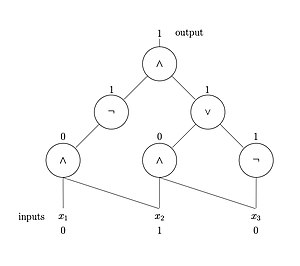
\includegraphics[scale=0.6]{booleanC.jpg}
\end{center}
\caption{Boolean circuit example \cite{booleanC}}
\end{figure}

\end{CountingDefinition}









%-------------------------------------------------------------

\subsection*{Reduction REACHABILITY PATH to CIRCUIT VALUE}

\begin{CountingDefinition}[Problem: GRAPH REACHABILITY]{def:validLabelPlacement}
Given a graph $G$ and two nodes $n_1, n_2 \in V$, is there  path from $n_1$ to $n_2$?

A graph $G=(V, E)$ is a finite set $V$ of nodes and a set $E$ of edges as node pairs.
\ \\

REACHIBILITY can be nondeterministically solved in space $\log n$.
\end{CountingDefinition}




\begin{CountingDefinition}[Problem: CIRCUIT VALUE]{def:validLabelPlacement}
The CIRCUIT VALUE Problem is the problem of computing the output of a given Boolean circuit on a given input.

In terms of time complexity, it can be solved in linear time (topological sort).


The problem is closely related to the SAT (Boolean Satisfiability) problem which is complete for NP and its complement, which is complete for co-NP.
\end{CountingDefinition}


\begin{itemize}
\item REACHABILITY can be reduced to CIRCUIT VALUE \\
$\rightarrow$ demonstrates REACHABILITY is not significantly harder that CIRCUIT VALUE
\item construct a variable-free circuit $R(G)$ that has \textit{true} as output only if $G$ has a path from the start node to node $n$ 
\item $R(x)$ uses no $\lnot$ gates (monotone circuit) 
\item (both problema are in P)
\item idea: use the Floyd-Warshall algorithm (dynamic programming)
\item instance: Graph $G = (V, E)$ with $n$ nodes $(1,2,...,n)$

\item the gates:
\begin{itemize}
\item $g_{i,j,k}$ with $1 \leq i, j \leq n$ and $0 \leq k \leq n$
\begin{itemize}
\item there is a path from node $i$ to node $j$ without passing through a node bigger than $k$
\item $g_{i,j,0}$ is true if and only if $i=j$ or $i$ and $j$ are neighbours
\end{itemize}
\item $h_{i,j,k}$ with $1 \leq i, j, k \leq n$
\begin{itemize}
\item there is a path from node $i$ to node $j$ passing through $k$ but not any node bigger than $k$
\end{itemize}

\end{itemize}

\item $h_{i,j,k}$ is an \textit{and} gate with predecessors $g_{i, k, k-1}$ and $g_{k, j, k-1}$ where $k= 1, 2, ..., n$
\item $g_{i, j, k}$ is an \textit{or} gate with predecessors $g_{i, j, k-1}$ and $h_{i, j, k}$ where $k = 1, 2, ... , n$
\item $g_{1,n,n}$ is the output gate

\item [] \cite{RCV}

\end{itemize}

\textbf{Proof idea:}



\color{red} TODO \\
proof \\
\color{black}
\color{violet} Questions:
\color{black}





%-------------------------------------------------------------

\subsection*{Reduction CIRCUIT SAT to SAT}

\begin{CountingDefinition}[Problem: CIRCUIT SAT]{def:validLabelPlacement}
The circuit satisfiability problem (CIRCUIT SAT) is the decision problem of determining whether a given Boolean circuit has an assignment of its inputs that makes the output true.
\end{CountingDefinition}

\begin{itemize}
\item CIRCUIT SAT can be reduced to SAT \\
$\rightarrow$ demonstrates CIRCUIT SAT is not significantly harder that SAT
\item 
given a circuit C, construct a boolean expression $R(C)$ such that $R(C)$ is satisfiable if and only if $C$ is satisfiable
% \item R(C) will turn out to be a CNF.
\item the variables of $R(C)$ are those of $C$ plus $g$ for each gate $g$ of $C$
\item clauses of $R(C)$:
\begin{itemize}
\item $g$ is a variable gate $x$: \\
Add clauses $(\lnot g \vee x)$ and $(g \vee \lnot x) \equiv g \Leftrightarrow x$
\item $g$ is a \textit{true} gate: \\
Add clause $(g)$ $\rightarrow$ $g$ must be true to make $R(C)$ true
\item $g$ is a \textit{false} gate: \\
Add clause $(\lnot g)$ $\rightarrow$ $g$ must be false to make $R(C)$ true
\item $g$ is a $\lnot$ gate with predecessor gate $h$: \\
Add clauses $(\lnot g \vee \lnot h)$ and $(g \vee h) \equiv g \Leftrightarrow \lnot h$ \\
\item $g$ is a $\vee$ gate with predecessor gates $h$ and $h'$: \\
Add clauses $(\lnot h \vee g)$, $(\lnot h' \vee g)$ and $(h \vee h' \vee \lnot g)$, meaning: $g \Leftrightarrow (h \vee h')$
\item $g$ is a $\wedge$ gate with predecessor gates $h$ and $h'$: \\
Add clauses $(\lnot g \vee h)$, $(\lnot g \vee h')$, and $(\lnot h \vee \lnot h' \vee g)$, meaning: $g \Leftrightarrow (h \wedge h')$
\item $g$ is the output gate: \\
Add clause $(g)$, meaning: $g$ must be true to make $R(C)$ true
\end{itemize}
\item[] \cite{RCV}
\end{itemize}

\textbf{Example:} \\
\begin{minipage}{0.4\textwidth}

\begin{figure}[H]
\begin{center}
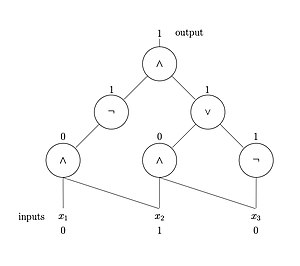
\includegraphics[scale=0.6]{booleanC.jpg}
\end{center}
\caption{Boolean circuit example \cite{booleanC}}
\end{figure}

\end{minipage}\begin{minipage}{0.6\textwidth}

\begin{itemize}
\item $g$ as variable gate: $\ \ \ x_1 \ \ \ \  x_2 \ \ \ \ \ x_3$
\item $g$ as $\wedge$ gate: $\ \ \ (x_1 \wedge x_2) \ \ \ \ \ (x_2 \wedge x_3)$
\item $g$ as $\lnot$ gate: $\ \ \ (\lnot x_3) \ \ \ \ \ \lnot (x_1 \wedge x_2)$
\item $g$ as $\vee$ gate: $\ \ \ (x_2 \wedge x_3) \vee \lnot x_3$
\item $g$ as $\wedge$ gate: $\ \ \ \lnot(x_1 \wedge x_2) \wedge ((x_2 \wedge x_3) \vee \lnot x_3)$
\end{itemize}

\end{minipage}

\ \\
\textbf{Proof idea:}






\color{red} TODO \\
proof idea \\
\color{black}
\color{violet} Questions:
\color{black}








%-------------------------------------------------------------

\subsection*{Generalization}

\begin{itemize}
\item generalizations are a special form of reductions 
\item problem $A$ is a generalization of problem $B$ if every instance of $B$ is also an instance of $A$
$\rightarrow$ $B$ can be reduced to $A$
\item inputs of $A$ are a subset of inputs of $B$ and on those inputs $A$ and $B$ have the same answers
\end{itemize}

\begin{CountingDefinition}[Generalization]{def:validLabelPlacement}
Problem $A$ is a generalization of problem $B$ if every instance of $B$ is also an instance of $A$. This implies $B$ can be reduced to $A$.

The inputs of $A$ are a subset of inputs of $B$ and on those inputs $A$ and $B$ have the same answers.
\end{CountingDefinition}









%-------------------------------------------------------------

\subsection*{Closedness under Composition}


\color{red} TODO \\
\color{black}
\color{violet} Questions:
\color{black}





\newpage

\printbibliography




\end{document}